\documentclass[10pt]{beamer}

\input{/Users/danielschreurs/Documents/LaTeX/beamer-style.tex.tex}

\title{Systèmes de Gestion de Bases de Données - 2e}
\subtitle{Chapitre 4 - Langage de Manipulation des données (LMD)}
\date{\today}
\author{Daniel Schreurs}
\institute{Haute École de Province de Liège}
%\titlegraphic{\hfill\includegraphics[height=1.5cm]{logo.eps}}


\setbeamertemplate{frame footer}{\insertsectionhead}

\begin{document}

\maketitle

\setbeamerfont{subsection in toc}{size=\small}
\setbeamerfont{subsubsection in toc}{size=\normalsize}
\setbeamertemplate{section in toc}[sections numbered]
\setbeamertemplate{subsection in toc}[subsections numbered]
\setbeamertemplate{subsubsection in toc}[subsubsections numbered]
\begin{frame}[allowframebreaks]{Table des matières du chapitre}
    \tableofcontents[subsectionstyle=show/show/hide,subsubsectionstyle=show/show/hide,]
\end{frame}

\section{Introduction}
\tocss
\subsection{Définition}
\begin{frame}{\secname : \subsecname}
    Un langage de manipulation des données, ou LMD, contient des commandes :
    \begin{itemize}
        \item d'interrogation (recherche)
        \item de modification.
    \end{itemize}
    Toutes ces commandes concernent toujours un ensemble de tuples qui satisfait un critère de qualification.
\end{frame}

\begin{frame}{\secname : \subsecname}
    En SQL :
    \begin{itemize}
        \item Commande d'interrogation : SELECT
        \item Commandes de modification :
              \begin{itemize}
                  \item ajout (INSERT),
                  \item mise à jour (UPDATE)
                  \item suppression (DELETE)
              \end{itemize}
    \end{itemize}
    Remarque : dans ce chapitre, la présentation des commandes de modification se fera sans tenir compte du concept de transaction (accès concurrents) qui sera abordé dans le chapitre 5.
\end{frame}

\subsection{Remarques}
\begin{frame}[allowframebreaks]{\secname : \subsecname}
    Quelques remarques à propos de l'écriture des requêtes SQL :
    \begin{itemize}
        \item SQL est insensible à la casse
        \item La syntaxe des commentaires est :
              \begin{itemize}
                  \item  \lstinline[language=sql]!--! : commentaire sur une seule ligne
                  \item  \lstinline[language=sql]!/* ... */! : commentaire sur plusieurs lignes
              \end{itemize}
        \item Les chaînes de caractères : "sont écrites entre simple quote, une apostrophe dans une chaîne est dédoublée"
        \item Les chaînes de caractères sont écrites entre simple quote, une apostrophe dans une chaîne est dédoublée
        \item Ex : \lstinline[language=sql]!'Il fait beau aujourd''hui'!
        \item  Si un élément de la base a pour nom un mot réservé, il faut le spécifier entre guillemets
              Ex : \lstinline[language=sql]!CREATE TABLE "TABLE" ( ... )!;
        \item Les noms des objets
              \begin{itemize}
                  \item ont une longueur maximale de 128 caractères\footnote{Pour plus d'informations, consultez la \href{https://docs.oracle.com/en/database/oracle/oracle-database/12.2/refrn/ALL_OBJECTS.html\#GUID-AA6DEF8B-F04F-482A-8440-DBCB18F6C976}{documentation}.}.
                  \item doivent commencer par une lettre, peuvent contenir les caractères a à z, 0 à 9, \$, \# et \_
              \end{itemize}
        \item L'opérateur AS sert à donner un nom à une colonne sélectionnée ou calculée dans une requête : \lstinline[language=sql]!SELECT COUNT(*) AS Nbre FROM Employes;!
    \end{itemize}
\end{frame}

\section{Recherche de base}
\tocss
\subsection{SELECT}
\begin{frame}{\secname : \subsecname}
    \lstinputlisting[language=bnf,title=Clause SELECT]{../exemples/Chapitre 4/select.bnf}
\end{frame}

\subsection{WHERE}
\begin{frame}{\secname : \subsecname}
    La clause WHERE permet de spécifier un critère de sélection.
    \lstinputlisting[language=bnf,title=Clause WHERE]{../exemples/Chapitre 4/where.bnf}
\end{frame}

\begin{frame}{\secname : \subsecname}
    Les possibilités de la clause WHERE sont étendues en développant la syntaxe de \lstinline[language=bnf]!condition\_de\_base!.
    \lstinputlisting[language=bnf,title=Condition de base]{../exemples/Chapitre 4/where2.bnf}
\end{frame}

\begin{frame}{\secname : \subsecname}
    SQL2 va plus loin dans la définition de la notion de \lstinline[language=sql]!condition_de_base! qui est appelée dans la norme comparison expression.
    \lstinputlisting[language=bnf,title=comparison expression]{../exemples/Chapitre 4/where3.bnf}
    \footnote{Une \lstinline[language=sql]!table\_expression! est une expression dont le résultat doit contenir au plus une ligne (selon la norme, une table ne contenant pas de lignes est convertie en une table contenant une ligne dont tous les éléments sont NULL).}
\end{frame}

\begin{frame}{\secname : \subsecname}
    \lstinputlisting[language=bnf,title=Exemples de row\_constructor]{../exemples/Chapitre 4/row-constructor.sql}
\end{frame}

\subsection{LIKE}
\begin{frame}{\secname : \subsecname}
    \lstinputlisting[language=bnf,title=L'opérateur LIKE permet de comparer des chaînes de caractères]{../exemples/Chapitre 4/like.bnf}
    \begin{itemize}
        \item \lstinline[language=sql]!\_! remplace un seul caractère
        \item \lstinline[language=sql]!\%! remplace un nombre quelconque (éventuellement \lstinline[language=sql]!NULL!) de caractères
    \end{itemize}
\end{frame}

\begin{frame}{\secname : \subsecname}
    \lstinputlisting[language=sql,title=Exemple : obtenir le nom des vues qui commencent par USER\_]{../exemples/Chapitre 4/like.sql}
\end{frame}

\begin{frame}{\secname : \subsecname}
    \lstinputlisting[language=sql,title=La comparaison tient compte de la longueur du type de la donnée]{../exemples/Chapitre 4/like2.sql}
    \begin{itemize}
        \item Aucun résultat !!!
        \item LIKE sans "joker"
        \item La comparaison tient compte de la longueur du type de la donnée
    \end{itemize}
\end{frame}

\begin{frame}{\secname : \subsecname}
    \lstinputlisting[language=sql,title=La comparaison tient compte de la longueur du type de la donnée]{../exemples/Chapitre 4/like3.sql}
    \begin{itemize}
        \item On obtient un résultat !
        \item Car on joue avec des \lstinline[language=sql]!VARCHAR! des deux côtés
    \end{itemize}
\end{frame}

\subsection{NULL}
\begin{frame}{\secname : \subsecname}
    \begin{itemize}
        \item \lstinline[language=sql]!NULL! est une absence de valeur
        \item Le résultat de la comparaison (\lstinline[language=sql]!<, <=, =, >=, >, <>!) entre \lstinline[language=sql]!NULL! et une autre valeur (même \lstinline[language=sql]!NULL!) n'est ni \textbf{VRAI} ni faux, mais inconnu
              Ex : \lstinline[language=sql]!NULL = NULL! ou \lstinline[language=sql]!NULL < NULL! vaut inconnu
    \end{itemize}
\end{frame}
\begin{frame}{\secname : \subsecname}
    \begin{figure}
        \begin{center}
            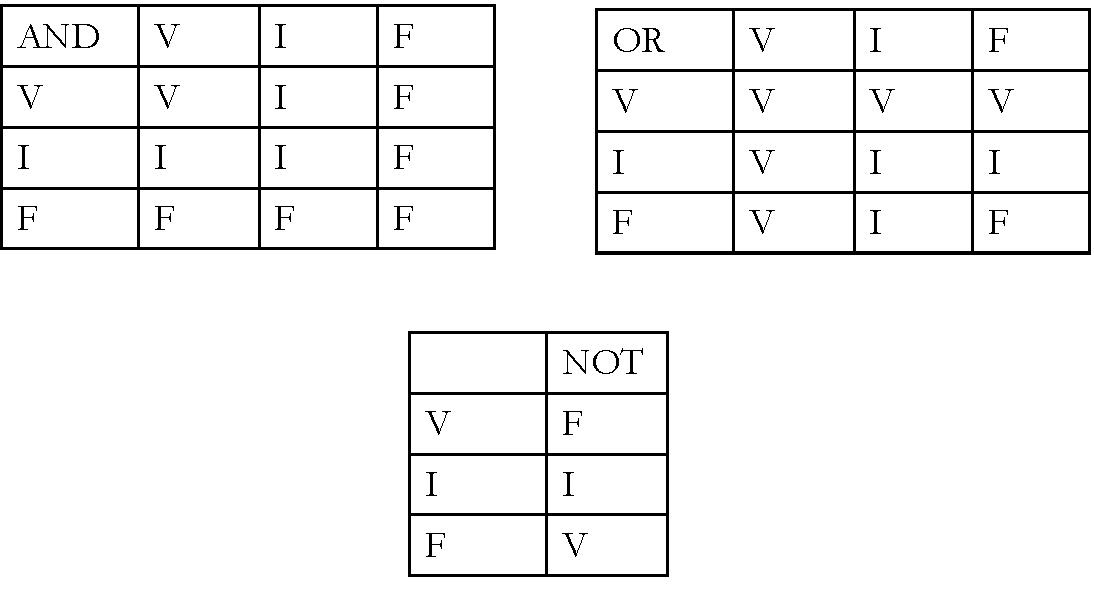
\includegraphics[width=0.60\textwidth]{../assets/img/table_verite.pdf}
            \caption{Tables de vérité : Vrai, faux, inconnu}
        \end{center}
    \end{figure}
\end{frame}
\begin{frame}{\secname : \subsecname}
    \lstinputlisting[language=bnf,title=Deux opérateurs spéciaux pour comparer une valeur à NULL]{../exemples/Chapitre 4/notin.sql}
\end{frame}

\begin{frame}{\secname : \subsecname}
    \lstinputlisting[language=bnf,title=COALESCE recherche la première valeur non NULL dans une liste de valeurs]{../exemples/Chapitre 4/coalesce.sql}
\end{frame}
\begin{frame}{\secname : \subsecname}
    \lstinputlisting[language=bnf,title=Tester si une valeur a été modifiée]{../exemples/Chapitre 4/coalesce2.sql}
\end{frame}

\subsection{Union}
\begin{frame}{\secname : \subsecname}
    Union, Intersection, différence :
    Les relations doivent être de même degré et les colonnes correspondantes doivent être compatibles
\end{frame}

\begin{frame}{\secname : \subsecname}
    \lstinputlisting[language=bnf,title=Union]{../exemples/Chapitre 4/union.bnf}
    \lstinline[language=bnf]!liste\_colonne! : $C_1, C_2, ... , C_n$!
    Chaque $C_i$ doit être présente à la fois dans les tables $A$ et $B$
\end{frame}

\begin{frame}{\secname : \subsecname}
    \lstinputlisting[language=sql,title=Exemple : rechercher le nom et le prénom des employées qui habitent dans la commune de Liège ou Waremme]{../exemples/Chapitre 4/union.sql}
    \begin{figure}
        \begin{center}
            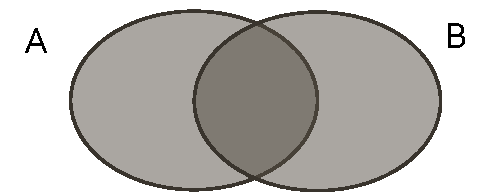
\includegraphics[width=0.3\textwidth]{../assets/img/union.pdf}
            \caption{union}
        \end{center}
    \end{figure}
\end{frame}
\subsection{EXCEPT}
\begin{frame}{\secname : \subsecname}
    \lstinputlisting[language=bnf,title=Différence]{../exemples/Chapitre 4/except.bnf}
    \lstinline[language=bnf]!liste\_colonne! : $C_1, C_2, ... , C_n$!
    Chaque $C_i$ doit être présente à la fois dans les tables $A$ et $B$
\end{frame}

\begin{frame}{\secname : \subsecname}
    \lstinputlisting[language=sql,title=Exemple : rechercher le numéro des employés qui n'ont pas de projets en cours]{../exemples/Chapitre 4/except.sql}
    \begin{figure}
        \begin{center}
            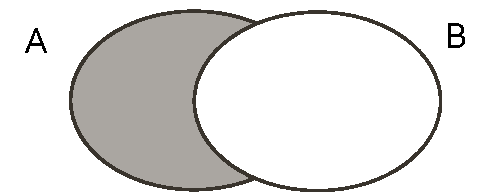
\includegraphics[width=0.3\textwidth]{../assets/img/difference.pdf}
            \caption{difference}
        \end{center}
    \end{figure}
\end{frame}

\subsection{INTERSECT}
\begin{frame}{\secname : \subsecname}
    \lstinputlisting[language=bnf,title=Différence]{../exemples/Chapitre 4/intersect.bnf}
    \lstinline[language=bnf]!liste\_colonne! : $C_1, C_2, ... , C_n$!
    Chaque $C_i$ doit être présente à la fois dans les tables $A$ et $B$
\end{frame}

\begin{frame}{\secname : \subsecname}
    \lstinputlisting[language=sql,title=Exemple : rechercher le numéro des employés qui travaillent sur les projets p10346 et p10349]{../exemples/Chapitre 4/intersect.sql}
    \begin{figure}
        \begin{center}
            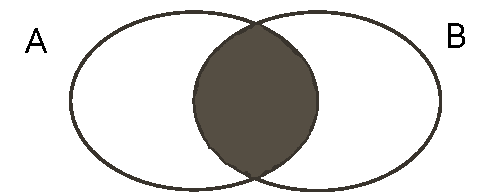
\includegraphics[width=0.3\textwidth]{../assets/img/intersection.pdf}
            \caption{intersection}
        \end{center}
    \end{figure}
\end{frame}

\begin{frame}{\secname : \subsecname}
    $$
        A \cap B = A - (A-B) = B- (B-A)
    $$
    \lstinputlisting[language=sql,title=Exemple : rechercher le numéro des employés qui travaillent sur les projets p10346 et p10349]{../exemples/Chapitre 4/intersect2.sql}
\end{frame}

\begin{frame}{\secname : \subsecname}
    \lstinputlisting[language=sql,title=Requêtes erronées]{../exemples/Chapitre 4/intersect3.sql}
\end{frame}

\begin{frame}{\secname : \subsecname}
    \lstinputlisting[language=sql,title=Exemple : Afficher le nom et le prénom des employés qui travaillent sur le projet p10346 et sur le projet p10349]{../exemples/Chapitre 4/intersect4.sql}
\end{frame}


\subsection{Exercices}
\begin{frame}{\secname : \subsecname}
    \begin{itemize}
        \item Afficher le numéro des départements composés uniquement de femmes, sachant que le numéro de département peut-être inconnu
        \item Afficher le numéro des départements composés d'hommes et de femmes, sachant que le numéro de département peut-être inconnu
        \item Afficher le numéro des départements composés d'employés habitant à Liège ou Herstal
        \item Afficher le numéro des employés qui ne dirigent personne, sachant qu'un chef de département doit être chef d'au moins un employé
    \end{itemize}
\end{frame}

\begin{frame}{\secname : \subsecname}
    \lstinputlisting[language=sql,title=Afficher le numéro des départements composés uniquement de femmes sachant que le numéro de département peut-être inconnu]{../exemples/Chapitre 4/ex1.sql}
\end{frame}

\begin{frame}{\secname : \subsecname}
    \lstinputlisting[language=sql,title=Afficher le numéro des départements composés d'hommes et de femmes sachant que le numéro de département peut-être inconnu]{../exemples/Chapitre 4/ex2.sql}
\end{frame}

\begin{frame}{\secname : \subsecname}
    \lstinputlisting[language=sql,title=Afficher le numéro des départements composés d'employés habitant à Liège ou Herstal]{../exemples/Chapitre 4/ex3.sql}
\end{frame}
\begin{frame}{\secname : \subsecname}
    \lstinputlisting[language=sql,title=Afficher le numéro des employés qui ne dirigent personne sachant qu'un chef de département doit être chef d'au moins un employé]{../exemples/Chapitre 4/ex4.sql}
\end{frame}

\section{Recherche de base avec jointure}
\tocss
\subsection{Jointure prédicative ou jointure manuelle}

\begin{frame}{\secname : \subsecname}
    \lstinputlisting[language=sql,title=Jointure prédicative ou jointure manuelle]{../exemples/Chapitre 4/join.sql}
\end{frame}

\begin{frame}{\secname : \subsecname}
    \lstinputlisting[language=sql,title=Jointure prédicative ou jointure manuelle]{../exemples/Chapitre 4/join2.sql}
    \footnote{4 tables impliquent 3 instructions de jointure manuelle !!!}
\end{frame}

\subsection{Jointure interne non-equijointure}
\begin{frame}{\secname : \subsecname}
    Une jointure avec une condition autre que l'égalité.
    Les conditions peuvent utiliser :
    \lstinline[language=sql]!\>\=   \<   \<\=   \<\>   IN   LIKE   BETWEEN   EXISTS!
    \lstinputlisting[language=sql,title=Donnez le nom des employés qui ont un salaire > à "BEART"
    ]{../exemples/Chapitre 4/join3.sql}
\end{frame}

\subsection{Auto-jointure}
\begin{frame}{\secname : \subsecname}
    \lstinputlisting[language=sql,title=Afficher le nom de l'employé ainsi que le nom de son chef direct]{../exemples/Chapitre 4/autojoin.sql}
\end{frame}


\begin{frame}{\secname : \subsecname}
    \lstinputlisting[language=sql,title=L'auto-jointure permet donc aussi d'implémenter l'intersection !]{../exemples/Chapitre 4/autojoin2.sql}
\end{frame}

\subsection{Jointure naturelle}
\begin{frame}{\secname : \subsecname}
    \begin{itemize}
        \item   La jointure s'effectue sur les colonnes communes, c'est-à-dire sur les colonnes qui portent le même nom\footnote{Même si l'information n'a rien à voir}.
        \item Le mot clé \lstinline[language=sql]!USING! permet de restreindre les colonnes communes à prendre en considération
        \item Une jointure naturelle peut être une jointure \lstinline[language=sql]!INNER!, \lstinline[language=sql]!LEFT OUTER! ou \lstinline[language=sql]!RIGHT OUTER!. La valeur par défaut est : \lstinline[language=sql]!INNER!.
    \end{itemize}
    \lstinputlisting[language=sql,title=L'auto-jointure permet donc aussi d'implémenter l'intersection !]{../exemples/Chapitre 4/naturaljoin.sql}
\end{frame}

\begin{frame}{\secname : \subsecname}
    \lstinputlisting[language=sql,title=Afficher le nom des employés ainsi que le numéro des projets qui leur sont affectés.]{../exemples/Chapitre 4/naturaljoin2.sql}
\end{frame}


\subsection{Jointure interne}

\begin{frame}{\secname : \subsecname}
    \lstinputlisting[language=sql,title=Afficher le nom des employés ainsi que le numéro des projets auxquels ils sont affectés]{../exemples/Chapitre 4/innerjoin.sql}
\end{frame}

\begin{frame}{\secname : \subsecname}
    \lstinputlisting[language=sql,title=Afficher le nom des employés ainsi que le NOM des projets auxquels ils sont affectés]{../exemples/Chapitre 4/innerjoin1.sql}
    \begin{figure}
        \begin{center}
            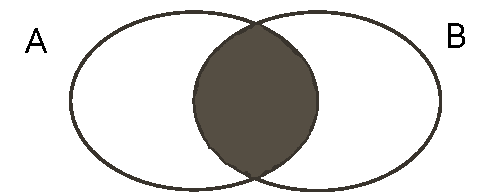
\includegraphics[width=0.3\textwidth]{../assets/img/intersection.pdf}
            \caption{intersection}
        \end{center}
    \end{figure}
\end{frame}

\subsection{Jointure externe}
\begin{frame}{\secname : \subsecname}
    La jointure externe permet de récupérer les lignes des tables correspondant au critère de jointure, mais aussi celles pour lesquelles il n'existe pas de correspondance.
    \lstinputlisting[language=sql,title=Jointure externe]{../exemples/Chapitre 4/left-join.sql}
    \begin{figure}
        \begin{center}
            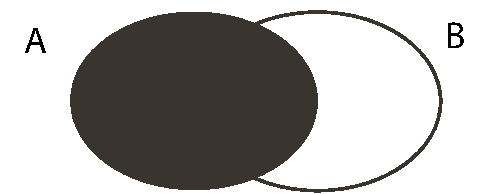
\includegraphics[width=0.3\textwidth]{../assets/img/left-join.pdf}
            \caption{Jointure externe gauche}
        \end{center}
    \end{figure}
\end{frame}
\begin{frame}{\secname : \subsecname}
    RIGHT OUTER : On cherche tous les tuples satisfaisant la condition de jointure précisée dans le prédicat, puis on rajoute toutes les lignes de la table TableDroite qui n'ont pas été prises en compte au titre de la satisfaction du critère.
    \begin{figure}
        \begin{center}
            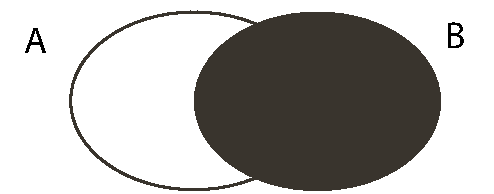
\includegraphics[width=0.3\textwidth]{../assets/img/right-join.pdf}
            \caption{Jointure externe droite}
        \end{center}
    \end{figure}
\end{frame}
\begin{frame}{\secname : \subsecname}
    LEFT OUTER : On cherche tous les tuples satisfaisant la condition de jointure précisée dans le prédicat, puis on rajoute toutes les lignes de la table TableGauche qui n'ont pas été prises en compte au titre de la satisfaction du critère.
    \begin{figure}
        \begin{center}
            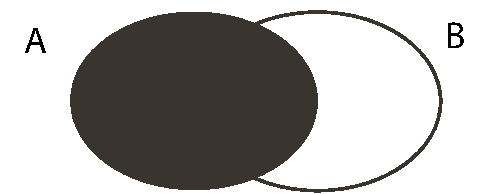
\includegraphics[width=0.3\textwidth]{../assets/img/left-join.pdf}
            \caption{Jointure externe gauche}
        \end{center}
    \end{figure}
\end{frame}

\begin{frame}{\secname : \subsecname}
    FULL OUTER : On cherche tous les tuples satisfaisant la condition de jointure précisée dans le prédicat, puis on rajoute toutes les lignes des tables TableGauche et TableDroite qui n'ont pas été prises en compte au titre de la satisfaction du critère.
    \begin{figure}
        \begin{center}
            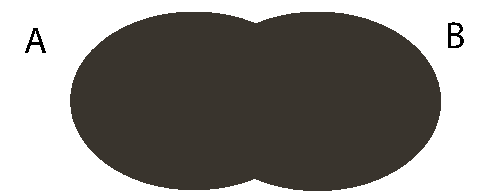
\includegraphics[width=0.3\textwidth]{../assets/img/full-join.pdf}
            \caption{Jointure externe gauche+droite}
        \end{center}
    \end{figure}
\end{frame}

\begin{frame}{\secname : \subsecname}
    \lstinputlisting[language=sql,title=Afficher le nom des employés ainsi que le numéro des projets auxquels ils sont affectés.]{../exemples/Chapitre 4/left-join-exemple.sql}
    \footnote{Attention aux employés qui n'ont pas de projets en cours.}
\end{frame}

\begin{frame}{\secname : \subsecname}
    \lstinputlisting[language=sql,title=Afficher le numéro et le nom des employés qui n'ont pas de projet en cours.]{../exemples/Chapitre 4/left-join-exemple1.sql}
\end{frame}

\begin{frame}{\secname : \subsecname}
    La jointure externe permet donc, entre autres, d'implémenter la différence :
    \lstinputlisting[language=sql,title=Afficher le numéro et le nom des employés qui n'ont pas de projet en cours.]{../exemples/Chapitre 4/left-join-exemple2.sql}
\end{frame}

\subsection{Jointure d'union}
\begin{frame}{\secname : \subsecname}
    Il n'y a pas de critère de jointure !
    \lstinputlisting[language=sql,title=La jointure d'union concatène les tables sans aucune correspondance de colonne]{../exemples/Chapitre 4/union-join.sql}
\end{frame}

\subsection{Remarque : clause FROM}
\begin{frame}{\secname : \subsecname}
    Extension de SQL2 : possibilité de placer une liste de \lstinline[language=bnf]!table-expression! dans la clause \lstinline[language=sql]!FROM!
    \lstinputlisting[language=sql,title=Exemple : afficher le nom des projets développés par l'employé DE NIRO]{../exemples/Chapitre 4/from.sql}
\end{frame}


\subsection{Exercices}
\begin{frame}{\secname : \subsecname}
    Exercices sur les jointures
    \begin{itemize}
        \item Rechercher le nom des employés et le nom du département dans lequel ils travaillent (le faire via une jointure manuelle, interne ; quid si on le fait avec une jointure naturelle ?)
        \item Rechercher les paires d'employés qui habitent la même commune
        \item Rechercher le nom des départements qui possèdent le même responsable
        \item Rechercher le nom des projets auxquels aucun employé n'est affecté
        \item Rechercher le nom des employés qui ne sont affectés à aucun projet
    \end{itemize}
\end{frame}
\begin{frame}[allowframebreaks]{\secname : \subsecname}
    \lstinputlisting[language=sql,title=Rechercher le nom des employés et le nom du département dans lequel ils travaillent (le faire via une jointure manuelle et interne. Quid si on le fait avec une jointure naturelle ?)]{../exemples/Chapitre 4/ex-join-1.sql}
\end{frame}

\begin{frame}{\secname : \subsecname}
    \lstinputlisting[language=sql,title=Rechercher les paires d'employés qui habitent la même commune]{../exemples/Chapitre 4/ex-join-2.sql}
\end{frame}
\begin{frame}{\secname : \subsecname}
    \lstinputlisting[language=sql,title=Rechercher le nom des départements qui possèdent le même responsable]{../exemples/Chapitre 4/ex-join-3.sql}
\end{frame}

\begin{frame}{\secname : \subsecname}
    \lstinputlisting[language=sql,title=Rechercher le nom des projets auxquels aucun employé n'est affecté]{../exemples/Chapitre 4/ex-join-4.sql}
\end{frame}

\begin{frame}{\secname : \subsecname}
    \lstinputlisting[language=sql,title=Rechercher le nom des employés qui ne sont affectés à aucun projet]{../exemples/Chapitre 4/ex-join-5.sql}
\end{frame}
\section{Expressions SQL}
\tocss
\subsection{Enrichir les clauses}
\begin{frame}{\secname : \subsecname}
    \begin{itemize}
        \item Enrichir les possibilités de la clause de sélection du \lstinline[language=sql]!SELECT! : \lstinline[language=bnf]!clause\_de\_selection ::=
              * | nom\_table.* | liste\_expression!
        \item Enrichir les possibilités de la clause \lstinline[language=SQL]!WHERE!
    \end{itemize}
    \lstinputlisting[language=bnf,title=Clause WHERE]{../exemples/Chapitre 4/where-expression.bnf}
\end{frame}

\begin{frame}{\secname : \subsecname}
    Où ?
    \begin{itemize}
        \item Dans la clause ORDER BY
        \item Dans l'expression SELECT
        \item Dans l'instruction UPDATE … SET
        \item Dans l'instruction INSERT … VALUES
        \item Dans la clause WHERE
    \end{itemize}
\end{frame}
\subsection{Expressions numériques}
\begin{frame}{\secname : \subsecname}
    \lstinputlisting[language=bnf,title=Expressions numériques]{../exemples/Chapitre 4/expression-numerique.bnf}
\end{frame}

\begin{frame}{\secname : \subsecname}
    \lstinputlisting[language=bnf,title=Expressions numériques]{../exemples/Chapitre 4/expression-numerique2.bnf}
\end{frame}

\begin{frame}[allowframebreaks]{\secname : \subsecname}
    Expressions numériques (fct de calcul) : \lstinline[language=sql]!COUNT!, \lstinline[language=sql]!SUM!, \lstinline[language=sql]!AVG!, \lstinline[language=sql]!MAX!, \lstinline[language=sql]!MIN!
    \begin{itemize}
        \item Dans la littérature anglo-saxone, ces fonctions sont appelées Aggregate functions.
        \item L'argument de \lstinline[language=sql]!SUM! et AVG doit toujours être de type numérique.
        \item L'argument de \lstinline[language=sql]!COUNT!, \lstinline[language=sql]!MAX! et \lstinline[language=sql]!MIN! peuvent être de type numérique, caractère ou date
        \item Toutes les valeurs indéfinies (\lstinline[language=sql]!NULL!) de la collection sont toujours éliminées avant l'application de la fonctions
              À l'exception de \lstinline[language=sql]!COUNT(*)! où toutes les valeurs indéfinies sont comptées.
        \item Si l'argument est la collection vide, \lstinline[language=sql]!COUNT! donne 0, les autres fonctions donnent \lstinline[language=sql]!NULL!
    \end{itemize}
\end{frame}
\begin{frame}{\secname : \subsecname}
    \lstinputlisting[language=sql,title=Expressions numériques]{../exemples/Chapitre 4/exemple-expression1.sql}
\end{frame}

\begin{frame}{\secname : \subsecname}
    \lstinputlisting[language=sql,title=Afficher le nom de l'employé qui gagne le plus et le nom de l'employé qui gagne le moins - avec l'opérateur ensembliste UNION]{../exemples/Chapitre 4/exemple-expression2.sql}
\end{frame}

\begin{frame}{\secname : \subsecname}
    \lstinputlisting[language=sql,title=Afficher le nom de l'employé qui gagne le plus et le nom de l'employé qui gagne le moins]{../exemples/Chapitre 4/exemple-expression3.sql}
\end{frame}
\subsection{Expressions caractères}
\begin{frame}{\secname : \subsecname}
    \lstinputlisting[language=bnf,title=Expressions caractères]{../exemples/Chapitre 4/expression-caractere.bnf}
\end{frame}

\begin{frame}[allowframebreaks]{\secname : \subsecname}
    \begin{itemize}
        \item \lstinline[language=sql]!concat(ch1, ch2)! : cette fonction est identique à ||.
        \item \lstinline[language=sql]!initcap(ch)! donne la chaîne ch dont le premier caractère a été converti en majuscules et les autres caractères en minuscules.
        \item \lstinline[language=sql]!lower(ch)! : cette fonction est identique à celle de la norme.
        \item \lstinline[language=sql]!lpad(ch1, x [, ch2])! construit une chaîne de x caractères en complétant le début de ch1 par le nombre adéquat de fois la chaîne ch2. Par défaut, ch2 est le caractère blanc.
        \item \lstinline[language=sql]!ltrim(ch1 [, ch2])! retire du début de ch1 toutes les occurrences de ch2. Par défaut ch2, est le caractère blanc.
        \item \lstinline[language=sql]!replace(ch1, ch2 [, ch3])! donne la chaîne ch1 dans laquelle toutes les occurrences de ch2 ont été remplacées par ch3
        \item \lstinline[language=sql]!rpad(ch1, x [, ch2])! construit une chaîne de x caractères en complétant la fin de ch1 par le nombre adéquat de fois la chaîne ch2. Par défaut ch2, est le caractère blanc.
        \item \lstinline[language=sql]!rtrim(ch1, ch2)! retire de la fin de ch1 toutes les occurrences de ch2. Par défaut ch2, est le caractère blanc.
        \item \lstinline[language=sql]!substr(ch, x [, y])! extrait de ch, à partir de la position x, une sous-chaîne de longueur y. Si y est omis, substr extrait la sous-chaîne jusqu’à la fin de ch.
        \item \lstinline[language=sql]!translate(ch1, ch2, ch3)! donne la chaîne ch1 dans laquelle toutes les occurrences de chaque caractère de ch2 ont été remplacées par le caractère correspondant de ch3.
        \item \lstinline[language=sql]!upper(ch)! : cette fonction est identique à celle de la norme.
        \item \lstinline[language=sql]!instr(ch1, ch2 [, x] [, y])! donne la position de ch2 dans ch1. La chaîne ch1 est parcourue à partir du xème caractère. Si y est précisé, instr donne la position de la yème occurrence de ch2 dans ch1.
              length(ch) est identique à \lstinline[language=bnf]!character\_length!.
    \end{itemize}
\end{frame}


\subsection{Opérateur CASE}
\begin{frame}{\secname : \subsecname}
    \lstinputlisting[language=bnf,title=Opérateur CASE]{../exemples/Chapitre 4/case.bnf}
\end{frame}

\begin{frame}{\secname : \subsecname}
    \lstinputlisting[language=sql,title=Rechercher le nom ainsi que la fourchette du salaire des employés dont le nom contient la lettre 'e' en deuxième position.]{../exemples/Chapitre 4/case-exemple.sql}\footnote{
        La fourchette du salaire vaut " < 70000", "entre 70000 et 79999", "entre 80000 et 89999" ou "> 90000".
        On affichera également le sexe, sous la forme "Féminin" ou "Masculin"}
\end{frame}

\subsection{Expression de dates et temps}
\begin{frame}{\secname : \subsecname}
    \lstinputlisting[language=bnf,title=Expression de dates et temps]{../exemples/Chapitre 4/temps.bnf}
\end{frame}

\begin{frame}{\secname : \subsecname}
    \begin{itemize}
        \item \lstinline[language=sql]!CURRENT\_DATE! donne la date du jour selon le format 'aaaa-mm-jj'
        \item \lstinline[language=sql]!CURRENT\_TIME! donne l'heure courante selon le format 'hh:mm:ss'
        \item \lstinline[language=sql]!CURRENT\_TIMESTAMP! donne la date du jour et l'heure courante : CURRENT\_DATE concaténée à \lstinline[language=sql]!CURRENT\_TIME!
        \item \lstinline[language=bnf]!EXTRACT ( champ FROM source )! Permet d'extraire la valeur numérique d'un champ d'une expression de type \lstinline[language=bnf]!date_temps! ou intervalle.
        \item Le paramètre champ peut valoir : \lstinline[language=sql]!YEAR!, \lstinline[language=sql]!MONTH!, \lstinline[language=sql]!DAY!, \lstinline[language=sql]!HOUR!, \lstinline[language=sql]!MINUTE!, \lstinline[language=sql]!SECOND!
    \end{itemize}
\end{frame}
\begin{frame}{\secname : \subsecname}
    \lstinputlisting[language=sql,title=Exemple : Rechercher le nom des employés nés dans les années 50]{../exemples/Chapitre 4/exemple-temps.sql}
\end{frame}

\begin{frame}{\secname : \subsecname}
    Lors d'une conversion de
    \begin{itemize}
        \item \lstinline[language=sql]!DATE! en \lstinline[language=sql]!TIMESTAMP!, la partie \lstinline[language=sql]!TIME! est initialisée à \lstinline[language=sql]!00:00:00.00!
              \lstinline[language=sql]!TIME! en \lstinline[language=sql]!TIMESTAMP!, la partie \lstinline[language=sql]!DATE! est initialisée à \lstinline[language=sql]!CURRENT\_DATE!
              \lstinline[language=sql]!TIMESTAMP! en \lstinline[language=sql]!TIME!, on laisse tomber la partie \lstinline[language=sql]!DATE!
    \end{itemize}
\end{frame}

\begin{frame}{\secname : \subsecname}

    \begin{itemize}
        \item  La fonction \lstinline[language=sql]!CAST! permet de convertir un numérique vers une donnée de type datetime (\lstinline[language=sql]!DATE!, \lstinline[language=sql]!TIME!, \lstinline[language=sql]!TIMESTAMP!) ou interval (année-mois ou jour-temps) : \lstinline[language=bnf]!CAST (expression AS type\_de\_donnée | domaine)!
        \item La fonction \lstinline[language=sql]!EXTRACT! permet d'extraire l'année, le mois, le jour, les heures, minutes, secondes d'une donnée de type datetime ou interval
    \end{itemize}
    \lstinputlisting[language=bnf,title=EXTRACT]{../exemples/Chapitre 4/extract.bnf}
\end{frame}

\begin{frame}{\secname : \subsecname}
    \lstinputlisting[language=sql,title=Exemple CAST]{../exemples/Chapitre 4/exemple-cast.sql}
\end{frame}

\begin{frame}{\secname : \subsecname}
    \lstinputlisting[language=sql,title=Redéfinir le format des dates]{../exemples/Chapitre 4/exemple-cast2.sql}
\end{frame}

\subsection{Temps et environnements distribués}
\begin{frame}{\secname : \subsecname}
    \begin{itemize}
        \item SQL2 donne un ensemble de spécifications permettant de gérer correctement les problèmes de temps dans un environnement distribué.
        \item L'idée de base est que chaque utilisateur mémorise le temps GMT (Greenwich Mean Time) mais qu'il peut le visualiser et l'utiliser comme son temps local
    \end{itemize}
\end{frame}

\begin{frame}{\secname : \subsecname}
    Voici par exemple comment deux utilisateurs situés respectivement à San Francisco et à Helsinki peuvent manipuler la table T définie de la manière suivante :
    \lstinputlisting[language=sql,title=Redéfinir le format des dates]{../exemples/Chapitre 4/time.sql}
\end{frame}

\begin{frame}{\secname : \subsecname}
    \begin{figure}
        \begin{center}
            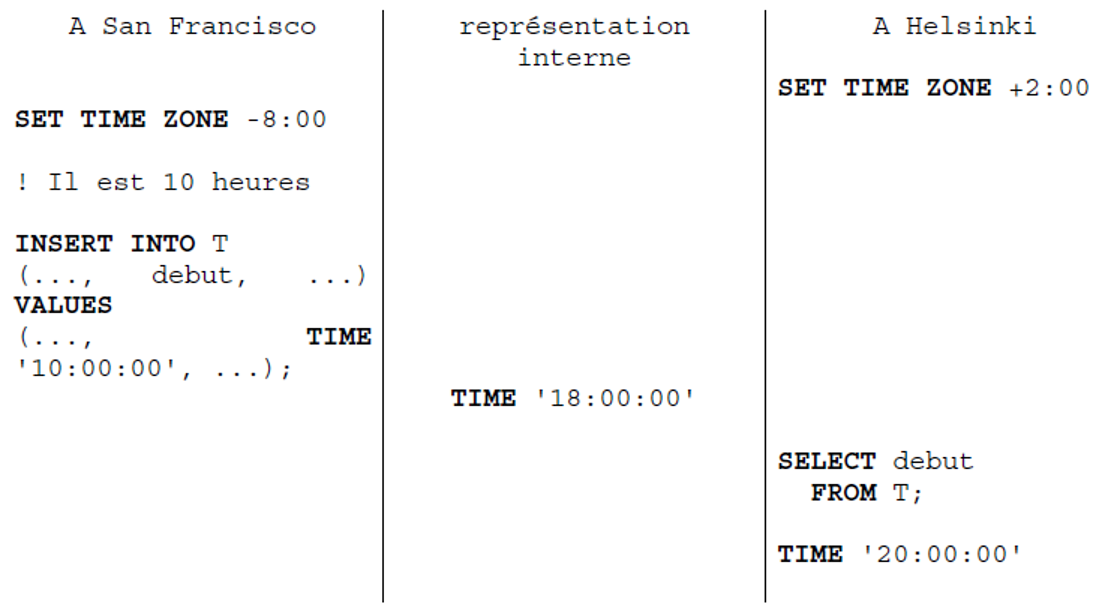
\includegraphics[width=0.85\textwidth]{../assets/img/time.png}
            \caption{Temps et environnements distribués}
        \end{center}
    \end{figure}
\end{frame}
\subsection{Expressions d'intervalles}
\begin{frame}{\secname : \subsecname}
    \begin{figure}
        \begin{center}
            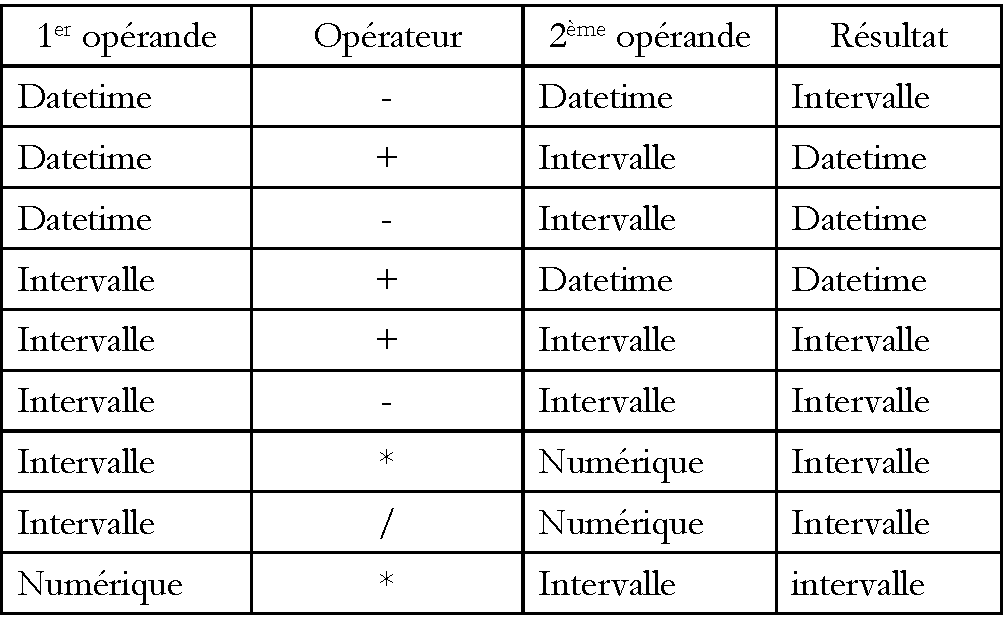
\includegraphics[width=0.85\textwidth]{../assets/img/expressions-intervalles.pdf}
            \caption{Opérations autorisées}
        \end{center}
    \end{figure}
\end{frame}

\begin{frame}[allowframebreaks]{\secname : \subsecname}
    \lstinputlisting[language=sql,title=Exemple : afficher l'âge des employés]{../exemples/Chapitre 4/exemple-intervalle.sql}\footnote{ATTENTION : le nombre d'années entre le 31/12/2018 et le 01/01/2019 vaut 1 !}
\end{frame}


\subsection{L'opérateur OVERLAPS}
\begin{frame}[allowframebreaks]{\secname : \subsecname}
    \begin{itemize}
        \item SQL2 possède un opérateur spécial : OVERLAPS.
        \item Overlaps permet de tester si deux périodes de temps se recouvrent.
              Ces périodes de temps peuvent être représentées de deux manières différentes : un temps de départ et un temps de fin ou un temps de départ et un intervalle.
        \item Pour plus d'info, voir les documents de référence.
    \end{itemize}
\end{frame}

\section{Tri}
\tocss
\subsection{Syntaxe}
\begin{frame}{\secname : \subsecname}
    \lstinputlisting[language=bnf,title=Tri]{../exemples/Chapitre 4/tri.bnf}
\end{frame}

\begin{frame}{\secname : \subsecname}
    \begin{itemize}
        \item Lors d'un tri, toutes les valeurs indéfinies (NULL) sont considérées comme étant identiques.
        \item Lors d'un tri, la valeur indéfinie (NULL) est considérée comme inférieure ou supérieur à toute valeur définie.  Ce choix est laissé au constructeur.
    \end{itemize}
    En Oracle, NULL est supérieure\footnote{On peut aussi préciser l'emplacement des NULL dans le résultat du tri en précisant NULL FIRST | NULL LAST} à toute valeur définie.
\end{frame}

\begin{frame}{\secname : \subsecname}
    \lstinputlisting[language=sql,title=Exemple : Afficher et trié par âge décroissant le nom des employés du départements 'Application telecom']{../exemples/Chapitre 4/exemple-tri.sql}
\end{frame}

\begin{frame}{\secname : \subsecname}
    \lstinputlisting[language=sql,title=Afficher et triés par commune le nom des employés habitant à Ans Neupré ou Chaudfontaine.  Les communes doivent apparaître dans l'ordre Neupré Ans puis Chaudfontaine.]{../exemples/Chapitre 4/exemple-tri2.sql}
\end{frame}

\section{Groupement de lignes}
\tocss
\subsection{Syntaxe}
\begin{frame}{\secname : \subsecname}
    \lstinputlisting[language=bnf,title=Groupement de lignes]{../exemples/Chapitre 4/group-by.bnf}
\end{frame}

\begin{frame}{\secname : \subsecname}
    \begin{itemize}
        \item Appelons $T$ le résultat de l'évaluation des clauses \lstinline[language=sql]!FROM!, \lstinline[language=sql]!WHERE!.
        \item Chaque colonne mentionnée dans la clause \lstinline[language=sql]!GROUP BY! doit être une colonne de $T$.
    \end{itemize}
\end{frame}

\begin{frame}{\secname : \subsecname}
    \begin{itemize}
        \item Le résultat de la clause \lstinline[language=sql]!GROUP BY! est une table intermédiaire constituée d'un ensemble de groupes de lignes issus de T de la manière suivante.
        \item Les lignes de $T$ sont (conceptuellement) réarrangées en groupes de telle sorte que dans chaque groupe toutes les lignes possèdent la même valeur pour la combinaison de colonnes indiquées dans la clause \lstinline[language=sql]!GROUP BY!.
        \item Chaque item de la clause \lstinline[language=sql]!SELECT! doit fournir une seule valeur par groupe : \lstinline[language=sql]!COUNT!, \lstinline[language=sql]!SUM!, \lstinline[language=sql]!AVG!, \lstinline[language=sql]!MAX! ou \lstinline[language=sql]!MIN!
    \end{itemize}
\end{frame}

\begin{frame}{\secname : \subsecname}
    \begin{itemize}
        \item \lstinline[language=sql]!HAVING! permet d'indiquer une condition qui sera évaluée pour chaque groupe formé en fonction de la clause \lstinline[language=sql]!GROUP BY!. Les groupes qui ne satisfont pas la condition sont éliminés.
        \item Les colonnes présentes dans la condition de la clause \lstinline[language=sql]!HAVING! doivent être présentes dans la clause \lstinline[language=sql]!GROUP BY!,  ou  argument d'une fonction,  ou être une référence externe .
    \end{itemize}
\end{frame}
\subsection{L'ordre d'évaluation}
\begin{frame}{\secname : \subsecname}
    \begin{enumerate}
        \item \lstinline[language=sql]!FROM!
        \item \lstinline[language=sql]!WHERE!
        \item \lstinline[language=sql]!GROUP BY!
        \item \lstinline[language=sql]!HAVING!
        \item \lstinline[language=sql]!SELECT!
        \item \lstinline[language=sql]!ORDER BY!
    \end{enumerate}
\end{frame}
\subsection{Exemples}
\begin{frame}{\secname : \subsecname}
    \lstinputlisting[language=sql,title=Exemple : Afficher le nombre d'employés par département]{../exemples/Chapitre 4/exemple-group-by.sql}
\end{frame}

\begin{frame}{\secname : \subsecname}
    \lstinputlisting[language=sql,title=Rechercher le nom le prénom et le nombre total d'heures hebdomadaires pour chaque employé et ce trié par nombre d'heures]{../exemples/Chapitre 4/exemple-group-by2.sql}
\end{frame}

\begin{frame}{\secname : \subsecname}
    \lstinputlisting[language=sql,title=Exemple : Rechercher le nom le prénom et le nombre total d'heures hebdomadaires pour les employés qui ont une charge < à 40 heures]{../exemples/Chapitre 4/exemple-group-by3.sql}
\end{frame}

\begin{frame}{\secname : \subsecname}
    \lstinputlisting[language=sql,title=Exemple : Rechercher le minimum d'heures hebdomadaires]{../exemples/Chapitre 4/exemple-group-by4.sql}
\end{frame}

\begin{frame}{\secname : \subsecname}
    \lstinputlisting[language=sql,title=Exemple : Rechercher le nom et le prénom des employés qui ont la plus petite charge hebdomadaire]{../exemples/Chapitre 4/exemple-group-by5.sql}
    Provoque une erreur à cause du \lstinline[language=xml]!MIN(SUM(heures))! Voir la solution au slide \ref{solution}.
\end{frame}


\begin{frame}{\secname : \subsecname}
    \lstinputlisting[label=solution,language=sql,title=Exemple : Rechercher le nom et le prénom des employés qui ont la plus petite charge hebdomadaire]{../exemples/Chapitre 4/exemple-group-by6.sql}\footnote{Pensez à ajouter les privilèges suffisants.\lstinline[language=sql]!GRANT CREATE ANY VIEW TO xx;!}
\end{frame}

\begin{frame}{\secname : \subsecname}
    Autre solution sans utiliser les vues :
    \lstinputlisting[language=sql,title=Exemple : Rechercher le nom et le prénom des employés qui ont la plus petite charge hebdomadaire]{../exemples/Chapitre 4/exemple-group-by7.sql}
\end{frame}

\begin{frame}{\secname : \subsecname}
    Autre solution sans utiliser les vues :
    \lstinputlisting[language=sql,title=Exemple : Afficher le maximum de la moyenne des salaires par département]{../exemples/Chapitre 4/exemple-group-by8.sql}
\end{frame}

\begin{frame}{\secname : \subsecname}
    Autre solution sans utiliser les vues :
    \lstinputlisting[language=sql,title=Exemple : Afficher le numéro de département qui a la moyenne des barèmes la plus élevée]{../exemples/Chapitre 4/exemple-group-by9.sql}
\end{frame}

\section{Sélections imbriquées}
\subsection{Pourquoi}
\begin{frame}{\secname : \subsecname}
    \begin{itemize}
        \item Les sélections imbriquées représentent un concept du SQL qui contribue grandement à sa puissance et à sa souplesse : la sélection imbriquée ou sous-question.
        \item Une sélection imbriquée n'est rien d'autre qu'un bloc de qualification SFW encapsulé à l'intérieur d'un autre bloc de qualification.
    \end{itemize}
\end{frame}

\subsection{Syntaxe}
\begin{frame}{\secname : \subsecname}
    \lstinputlisting[language=bnf,title=Sélections imbriquées]{../exemples/Chapitre 4/imbrication.bnf}
\end{frame}

\subsection{Syntaxe}
\begin{frame}{\secname : \subsecname}
    \lstinline[language=bnf]!condition\_in ::= expression [ NOT ] IN (sélection\_une\_colonne)!
    \newline

    Le résultat de l'évaluation de la condition \lstinline[language=bnf]!condition\_in! est \textbf{VRAI} si et seulement si la valeur de l'expression à gauche du \lstinline[language=sql]!IN! est égale à au moins une des valeurs du résultat du \lstinline[language=bnf]!sélection\_une\_colonne!.
\end{frame}

\subsection{Exemples}
\begin{frame}{\secname : \subsecname}
    \lstinputlisting[language=sql,title=Exemple : Rechercher le nom et le prénom des employés qui travaillent sur le projet p10347]{../exemples/Chapitre 4/exemple-imbrication1.sql}
\end{frame}

\begin{frame}{\secname : \subsecname}
    \lstinputlisting[language=sql,title=Exemple : Afficher le numéro des employés qui travaillent sur les projets 'p10346' et 'p10349']{../exemples/Chapitre 4/exemple-imbrication2.sql}
\end{frame}

\begin{frame}{\secname : \subsecname}
    \lstinputlisting[language=sql,title=Exemple : Afficher le numéro des employés qui n'ont pas de projets en cours]{../exemples/Chapitre 4/exemple-imbrication3.sql}
\end{frame}

\begin{frame}{\secname : \subsecname}
    \lstinputlisting[language=sql,title=Exemple : Rechercher le nom des départements qui n'ont pas d'employé qui gagne moins de 60000]{../exemples/Chapitre 4/exemple-imbrication4.sql}
\end{frame}

\begin{frame}{\secname : \subsecname}
    \metroset{block=fill}
    \begin{alertblock}{Important}
        \begin{itemize}
            \item Dans \lstinline[language=sql]!Employes! il existe des employés sans numéro de département et donc la requête imbriquée donne un numéro de département et \lstinline[language=sql]!NULL!
            \item Quand on fait la comparaison avec \lstinline[language=sql]!NULL! dans le \lstinline[language=sql]!NOT IN!, on obtient des résultats incorrects !
        \end{itemize}
    \end{alertblock}
\end{frame}

\begin{frame}{\secname : \subsecname}
    \lstinputlisting[language=sql,title=Exemple : Rechercher le nom des départements qui n'ont pas d'employé qui gagne moins de 60000]{../exemples/Chapitre 4/exemple-imbrication5.sql}
\end{frame}

\begin{frame}{\secname : \subsecname}
    \lstinputlisting[language=sql,title=Exemple : Rechercher le nom et le prénom des employés qui travaillent 10 heures sur le projet p10349]{../exemples/Chapitre 4/exemple-imbrication6.sql}
\end{frame}

\subsection{Remarques}
\begin{frame}{\secname : \subsecname}
    \lstinline[language=bnf]!condition\_all\_any ::=expression oper\_comp [ ALL | ANY | SOME ] ( sélection\_une\_colonne )!
    Le résultat de l'évaluation de \lstinline[language=bnf]!oper\_comp ALL! est \textbf{VRAI} uniquement dans un des deux cas suivants :
    \begin{itemize}
        \item La comparaison indiquée par \lstinline[language=bnf]!oper\_comp! est VRAIE pour toutes les valeurs du résultats du \lstinline[language=bnf]!selection\_une\_colonne!
        \item Le résultat du \lstinline[language=bnf]!selection\_une\_colonne! est vide
    \end{itemize}
\end{frame}

\begin{frame}{\secname : \subsecname}
    \lstinline[language=bnf]!condition\_all\_any ::= expression oper\_comp [ ALL | ANY | SOME ] ( sélection\_une\_colonne )!
    Le résultat de l'évaluation de \lstinline[language=bnf]!oper\_comp ANY (SOME)! est \textbf{VRAI} si et seulement si la comparaison indiquée par \lstinline[language=bnf]!oper\_comp! est VRAIE pour au moins une des valeurs du résultat du \lstinline[language=bnf]!selection\_une\_colonne!.
\end{frame}

\begin{frame}{\secname : \subsecname}
    \lstinline[language=bnf]!condition\_all\_any ::= expression oper\_comp [ ALL | ANY | SOME ] ( sélection\_une\_colonne )!
    \begin{itemize}
        \item  Le résultat de l'évaluation de \lstinline[language=bnf]!oper\_comp ANY (SOME)! est \textbf{FAUX} si la comparaison indiquée par \lstinline[language=bnf]!oper\_comp! est FAUSSE pour chaque valeur du résultat du \lstinline[language=bnf]!selection_une_colonne!.
        \item Dans tous les autres cas, le résultat de \lstinline[language=bnf]!oper_comp ANY (SOME)! est INCONNU
    \end{itemize}
\end{frame}

\subsection{Exemples}
\begin{frame}{\secname : \subsecname}
    \lstinputlisting[language=sql,title=Exemple : Afficher le numéro des employés qui travaillent sur les projets p10346 et p10349]{../exemples/Chapitre 4/exemple-imbrication7.sql}
\end{frame}

\begin{frame}{\secname : \subsecname}
    \lstinputlisting[language=sql,title=Exemple : Afficher le numéro des employés qui n'ont pas le plus petit salaire]{../exemples/Chapitre 4/exemple-imbrication8.sql}
\end{frame}

\begin{frame}{\secname : \subsecname}
    \lstinputlisting[language=sql,title=Exemple : Afficher le numéro des employés qui n'ont pas de projet en cours]{../exemples/Chapitre 4/exemple-imbrication9.sql}
\end{frame}

\begin{frame}{\secname : \subsecname}
    \lstinputlisting[language=sql,title=Exemple : Afficher le numéro des employés qui gagnent plus que tous les employés du département d00002]{../exemples/Chapitre 4/exemple-imbrication10.sql}
\end{frame}

\begin{frame}{\secname : \subsecname}
    \lstinputlisting[language=sql,title=Exemple : Afficher le nom des employés qui ont le salaire le plus élevé]{../exemples/Chapitre 4/exemple-imbrication11.sql}
\end{frame}

\begin{frame}{\secname : \subsecname}
    \lstinputlisting[language=sql,title=Exemple : Afficher le nom et le prénom des employés qui ont la plus petite charge hebdomadaire]{../exemples/Chapitre 4/exemple-imbrication12.sql}
\end{frame}

\begin{frame}{\secname : \subsecname}
    \lstinputlisting[language=sql,title=Exemple : Afficher le nom et le prénom des employés qui ont la plus petite charge hebdomadaire]{../exemples/Chapitre 4/exemple-imbrication13.sql}
\end{frame}

\subsection{Sous-requêtes corrélées}
\begin{frame}{\secname : \subsecname}
    \metroset{block=fill}
    \begin{alertblock}{Important}
        \begin{itemize}
            \item Il existe des requêtes pour lesquelles la sous question référence le niveau externe.
            \item Dans ce type de requêtes, il est impossible d'obtenir le résultat de la sous-question sans faire référence au niveau externe.
            \item On parle de \textbf{sous questions corrélatives}.
        \end{itemize}
    \end{alertblock}
\end{frame}

\subsection{Exemples}
\begin{frame}{\secname : \subsecname}
    \lstinputlisting[language=sql,title=Exemple : Afficher le nom et le prénom des employés qui ont travaillé 10 heures sur le projet p10349]{../exemples/Chapitre 4/exemple-imbrication14.sql}
\end{frame}


\begin{frame}{\secname : \subsecname}
    \metroset{block=fill}
    \begin{alertblock}{Important}
        \begin{enumerate}
            \item Le SGBD examine la première ligne de la table Employes.
            \item La variable \lstinline[language=sql]!Employes.NumSecu! vaut : 451278
            \item Le système évalue le bloc interne : \lstinline[language=sql]!(SELECT Heures, NumPro FROM EmpPro WHERE EmpPro.NumSecu = 451278);!
            \item $\{(10, p10345), (12, p10346), \boldsymbol{(10, p10349)}, (8, p10351)\}$
            \item L'employé 451278, Célarié Clémentine fait donc partie de la réponse.
            \item Le système répète le traitement pour toutes les lignes de la table employés.
        \end{enumerate}
    \end{alertblock}
\end{frame}

\begin{frame}{\secname : \subsecname}
    \lstinputlisting[language=sql,title=Exemple : Rechercher le nom des employés qui ne sont pas attachés au même département que leur chef]{../exemples/Chapitre 4/exemple-imbrication15.sql}
\end{frame}

\begin{frame}{\secname : \subsecname}
    \lstinputlisting[language=sql,title=Exemple : Rechercher le nom et le prénom des employés dont le salaire est supérieur au salaire moyen de leur département]{../exemples/Chapitre 4/exemple-imbrication16.sql}
\end{frame}

\begin{frame}{\secname : \subsecname}
    \lstinputlisting[language=sql,title=Exemple : Rechercher le nom et le prénom des employés qui ont travaillé 10 heures sur le projet p10349]{../exemples/Chapitre 4/exemple-imbrication17.sql}
\end{frame}

\begin{frame}{\secname : \subsecname}
    \lstinputlisting[language=sql,title=Exemple : Rechercher le numéro des employés qui ont travaillé sur les projets p10346 et p10349]{../exemples/Chapitre 4/exemple-imbrication18.sql}
\end{frame}

\begin{frame}{\secname : \subsecname}
    \lstinputlisting[language=sql,title=Exemple : Rechercher le numéro des employés qui n'ont pas de projet en cours]{../exemples/Chapitre 4/exemple-imbrication19.sql}
\end{frame}

\begin{frame}{\secname : \subsecname}
    \lstinputlisting[language=sql,title=Exemple : Rechercher le nom et le prénom des employés qui ont la plus petite charge hebdomadaire]{../exemples/Chapitre 4/exemple-imbrication20.sql}
\end{frame}

\section{Utilisation de "EXISTS"}
\tocss
\subsection{Tester l'existence de données}

\begin{frame}{\secname : \subsecname}
    Tester l'existence de données
    \begin{itemize}
        %\item Éviter l'utilisation des opérateurs ALL et ANY lorsque l'on ignore l'éventuelle présence de la valeur \lstinline[language=sql]!NULL!
        \item \lstinline[language=bnf]!condition\_exists ::= EXISTS (selection\_une\_colonne)!
        \item La valeur de \lstinline[language=bnf]!condition\_exists! est \textbf{VRAIE} si et seulement si l'évaluation de \lstinline[language=bnf]!sélection\_une\_colonne! n'est pas vide.  Sinon, la valeur de \lstinline[language=bnf]!condition\_exists! est \textbf{FAUSSE}
        \item L'opérateur \lstinline[language=sql]!EXISTS! est de loin l'opérateur le plus puissant de SQL
        \item On peut exprimer des jointures
        \item On peut réaliser des intersections, différences, divisions
    \end{itemize}
\end{frame}

\subsection{Exemples}
\begin{frame}{\secname : \subsecname}
    \lstinputlisting[language=sql,title=Exemple : Rechercher le nom et le prénom des employés qui ont travaillé 10 heures sur le projet p10349]{../exemples/Chapitre 4/exemple-exist.sql}
\end{frame}

\begin{frame}{\secname : \subsecname}
    \lstinputlisting[language=sql,title=Exemple : Rechercher le numéro des employés qui ont travaillé sur les projets p10346 et p10349]{../exemples/Chapitre 4/exemple-exist2.sql}
\end{frame}

\begin{frame}{\secname : \subsecname}
    \lstinputlisting[language=sql,title=Exemple : Rechercher le numéro des employés qui ne sont attachés à aucun projet]{../exemples/Chapitre 4/exemple-exist3.sql}
\end{frame}

\begin{frame}{\secname : \subsecname}
    \lstinputlisting[language=sql,title=Exemple : Rechercher le nom des départements qui ont au moins un employé qui gagne plus de 90000]{../exemples/Chapitre 4/exemple-exist4.sql}\footnote{Images Numeriques est un département qui n'a pas d'employés => ne devrait pas apparaître dans le résultat !}
\end{frame}

\begin{frame}{\secname : \subsecname}
    \lstinputlisting[language=sql,title=Exemple : Rechercher le nom des départements qui n'ont aucun employé qui gagne plus de 90000]{../exemples/Chapitre 4/exemple-exist5.sql}
\end{frame}

\begin{frame}{\secname : \subsecname}
    \lstinputlisting[language=sql,title=Exemple : Afficher le nom des employés qui ont le salaire le plus élevé]{../exemples/Chapitre 4/exemple-exist6.sql}\footnote{L'employé MONROE a un salaire inconnu $\implies$ ne devrait pas apparaître dans le résultat. Mais avec NOT EXISTS, la condition est vraie si le résultat de la sélection est vide !}
\end{frame}

\begin{frame}{\secname : \subsecname}
    \lstinputlisting[language=sql,title=Exemple : Afficher le nom des employés qui ont le salaire le plus élevé]{../exemples/Chapitre 4/exemple-exist7.sql}
\end{frame}
\begin{frame}{\secname : \subsecname}
    Exercices récapitulatifs :
    \begin{itemize}
        \item Afficher le numéro des employés qui travaillent sur les projets p10346 et p10349
        \item écrire de 6 manières différentes :
              \begin{itemize}
                  \item opérateur ensembliste;
                  \item auto-jointure;
                  \item requête imbriquée;
                  \item ALL/ANY/SOME;
                  \item EXISTS;
                  \item requête corrélée sans EXISTS.
              \end{itemize}
    \end{itemize}
\end{frame}

\begin{frame}{\secname : \subsecname}
    Exercices récapitulatifs :
    \begin{itemize}
        \item Afficher le numéro des employés qui n'ont pas de projet en cours
        \item écrire de 6 manières différentes :
              \begin{itemize}
                  \item opérateur ensembliste;
                  \item auto-jointure;
                  \item requête imbriquée;
                  \item ALL/ANY/SOME;
                  \item EXISTS;
                  \item requête corrélée sans EXISTS.
              \end{itemize}
    \end{itemize}
\end{frame}
\section{Mise à jour des données}
\tocss
\subsection{INSERT}
\begin{frame}{\secname : \subsecname}
    \lstinputlisting[language=bnf,title=INSERT]{../exemples/Chapitre 4/insert.bnf}
\end{frame}

\begin{frame}{\secname : \subsecname}
    \lstinputlisting[language=sql,title=On souhaite ajouter un nouveau département - Il s'agit du département "Infographie" dont on ne connaît pas le chef.]{../exemples/Chapitre 4/exemple-insert.sql}\footnote{Remarque : les colonnes pour lesquelles on ne spécifie pas explicitement une valeur sont initialisées à leur valeur par défaut.}
\end{frame}

\begin{frame}{\secname : \subsecname}
    \lstinputlisting[language=sql,title=Exemple : Insertion d'un employé]{../exemples/Chapitre 4/exemple-insert2.sql}
\end{frame}

\begin{frame}{\secname : \subsecname}
    Insérer l'employé DUBOIS, Luc.  Ce nouvel employé est attaché au département où il y a le moins d'employés, il a le barème moyen des employés et a pour chef son ami HOFFMAN
\end{frame}

\begin{frame}{\secname : \subsecname}
    \lstinputlisting[language=sql,title=Exemple : Insérer l'employé DUBOIS Luc]{../exemples/Chapitre 4/exemple-insert3.sql}
\end{frame}
\subsection{UPDATE}
\begin{frame}{\secname : \subsecname}
    \lstinputlisting[language=bnf,title=UPDATE]{../exemples/Chapitre 4/update.bnf}
\end{frame}

\begin{frame}{\secname : \subsecname}
    \lstinputlisting[language=sql,title=Exemple : Augmenter de 10\% le barèmes des employés du département 'Applications telecom']{../exemples/Chapitre 4/exemple-update.sql}
\end{frame}

\begin{frame}{\secname : \subsecname}
    \lstinputlisting[language=sql,title=Exemple : Attribuer à DE NIRO le salaire maximum du département auquel il est attaché]{../exemples/Chapitre 4/exemple-update2.sql}
\end{frame}

\subsection{DELETE}
\begin{frame}{\secname : \subsecname}
    \lstinputlisting[language=bnf,title=DELETE]{../exemples/Chapitre 4/delete.bnf}
\end{frame}

\begin{frame}{\secname : \subsecname}
    \lstinputlisting[language=sql,title=Exemple : Supprimer toutes les attributions de Clémentine CELARIE à un projet
    ]{../exemples/Chapitre 4/exemple-delete.sql}
\end{frame}
\end{document}